% ----------------------------------------------------------
% APÊNDICE A - Algoritmos
% ----------------------------------------------------------
\begin{apendicesenv}
\chapter{Algoritmos}
    \label{app:algoritmos}
	O algoritmo BinomialDistribution\_PROB tem como resultado a probabilidade de distribuição de um range e utiliza a fórmula  da probabilidade binomial geral abaixo. Esse algoritmo tem o mesmo resultado do algoritmo Distribution\_PROB, porém a execução do BinomialDistribution\_PROB é muito mais rápida e tem maior capacidade por usar números grandes como o BigInteger e o BigDecimal. Ambos os algoritmos foram feitos em C\# com o LINQPad 5 \footnotemark. Na Figura \ref{fig:BinomialDistribution_PROB_and_Distribution_PROB} é mostrado o resultado dos algoritmos para o range de 0 a 10, análogo ao lançamento de 10 moedas ao chão e somado os valores de caras e coras, sendo, por exemplo, a coroa com o valor um e a cara o valor dois. O algoritmo Distribution\_PROB soma cada uma das 1024 possibilidades [1,1,1,1,1,1,1,1,1,1 - 1,1,1,1,1,1,1,1,1,2 - ....] e agrupa esses valores somados. No algoritmo Distribution\_PROB esse conjunto de possibilidades é um produto cartesiano das possíveis combinações, o que torna esse algoritmo lento rapidamente, porém ele é importante para validar e facilitar o entendimento da a fórmula da probabilidade binomial geral utilizada no algoritmo BinomialDistribution\_PROB \cite{mathisfun_binomial_distribution}. Na Figura \ref{fig:BinomialDistribution_PROB_and_Distribution_PROB}, a tabela no interior de  Distribution\_PROB mostra esse agrupamento e o total de possibilidades, 1024. Ao dividir cada valor agrupado pelo total tem-se o resultado probabilístico alcançado pela fórmula empregada no BinomialDistribution\_PROB. Por exemplo, a probabilidade do somatório das 10 moedas lançadas ser 12 é igual a 45/1024, que é 0,0439453125 ou 4,39\%.
\footnotetext{O LINQPad 5 é encontrado em \url{www.linqpad.net} e pode ser utilizado em sua versão livre, Standard edition, sem expiração.}
\begin{align*}
f(k;n,p) &= \binom{n}{k} p^k(1 - p)^{n-k}
\end{align*}

\begin{figure}[H]
\caption{Resultado dos algoritmos  BinomialDistribution\_PROB e Distribution\_PROB}
\label{fig:BinomialDistribution_PROB_and_Distribution_PROB}
\centering
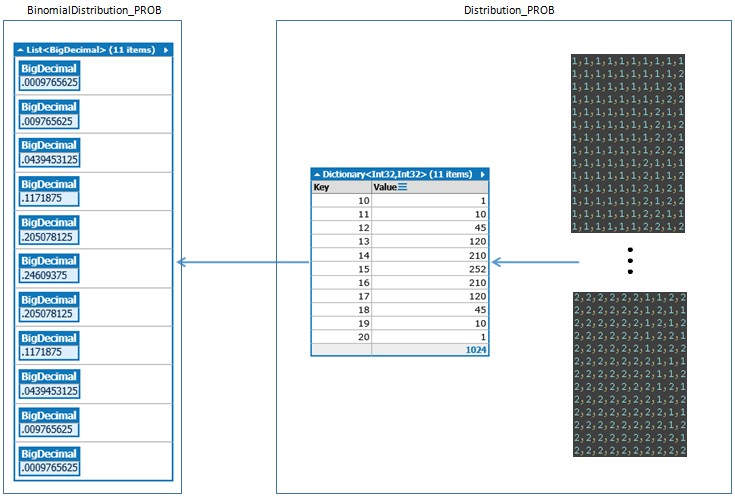
\includegraphics[scale=.75]{sections/images/BinomialDistribution_PROB_and_Distribution_PROB.jpg}
\floatfoot{O algoritmo Distribution\_PROB tem o intuito que clarificar a essência probabilística do teorema central do limite.} %\footnotemark.
\end{figure}

O algoritmo Distribution\_PROB também pode ser utilizado para o lançamento de 5 dados de 6 lados ou 6 dados de 5 lados, por exemplo. Como pode ser observado na Figura abaixo, a distribuição das probabilidades no lance dos dados é semelhante à distribuição binomial, das moedas.

\begin{figure}[H]
\centering
	\begin{subfigure}[H]{0.47\linewidth}
	\centering
	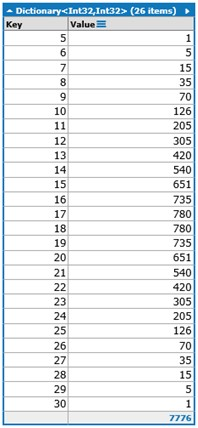
\includegraphics[width=.7\linewidth]{sections/images/Distribution_PROB_5_6.jpg}
	\caption{5 dados de 6 lados}
	\label{fig:Distribution_PROB_5_6}
	\end{subfigure}
\hfill
	\begin{subfigure}[H]{0.47\linewidth}
	\centering
	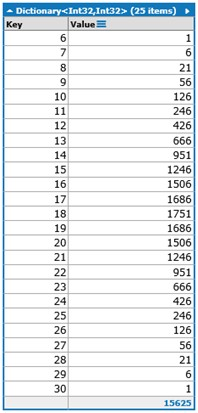
\includegraphics[width=.72\linewidth]{sections/images/Distribution_PROB_6_5.jpg}
	\caption{6 dados de 5 lados}
	\label{fig:Distribution_PROB_6_5}
	\end{subfigure}%
\caption{Resultados do algoritmo Distribution\_PROB}

\floatfoot{A distribuição das probabilidades no lance dos dados é consonante à distribuição binomial.} %\protect\footnotemark
\end{figure}

\end{apendicesenv}